\documentclass[preview]{standalone}
\usepackage{amsmath}
\usepackage{tikz}
\usepackage{mathdots}
\usepackage{yhmath}
\usepackage{cancel}
\usepackage{color}
\usepackage{xcolor}
\usepackage{siunitx}
\usepackage{array}
\usepackage{multirow}
\usepackage{amssymb}
\usepackage{gensymb}
\usepackage{tabularx}
\usepackage{extarrows}
\usepackage{booktabs}
\usetikzlibrary{fadings}
\usetikzlibrary{patterns}
\usetikzlibrary{shadows.blur}
\usetikzlibrary{shapes}
\begin{document}
\begin{center}



\tikzset{every picture/.style={line width=0.75pt}} %set default line width to 0.75pt        

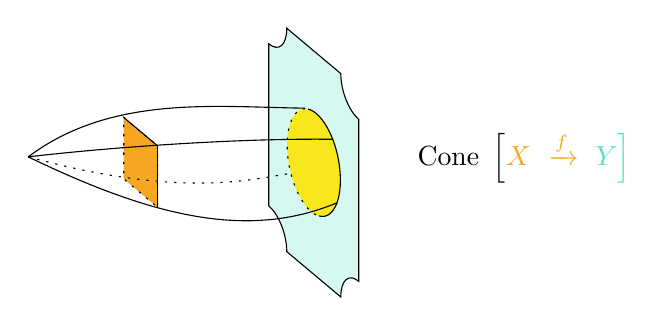
\begin{tikzpicture}[x=0.75pt,y=0.75pt,yscale=-1,xscale=1]
%uncomment if require: \path (0,158); %set diagram left start at 0, and has height of 158

%Shape: Plaque [id:dp5201993590706961] 
\draw  [fill={rgb, 255:red, 80; green, 227; blue, 194 }  ,fill opacity=0.24 ] (291.55,23) .. controls (296.35,27.02) and (300.23,23.66) .. (300.23,15.49) -- (326.25,37.33) .. controls (326.25,45.5) and (330.14,55.37) .. (334.93,59.39) -- (334.93,137.46) .. controls (330.14,133.44) and (326.25,136.8) .. (326.25,144.96) -- (300.23,123.13) .. controls (300.23,114.96) and (296.35,105.09) .. (291.55,101.07) -- cycle ;
%Shape: Arc [id:dp740636676918955] 
\draw  [draw opacity=0][fill={rgb, 255:red, 248; green, 231; blue, 28 }  ,fill opacity=1 ][dash pattern={on 0.84pt off 2.51pt}] (324.42,99.6) .. controls (324.42,99.6) and (324.42,99.6) .. (324.42,99.6) .. controls (320.95,109.13) and (313.14,108.19) .. (306.96,97.49) .. controls (300.78,86.79) and (298.59,70.39) .. (302.06,60.86) .. controls (304.11,55.21) and (307.7,53.24) .. (311.56,54.8) -- (313.24,80.23) -- cycle ; \draw  [dash pattern={on 0.84pt off 2.51pt}] (324.42,99.6) .. controls (324.42,99.6) and (324.42,99.6) .. (324.42,99.6) .. controls (320.95,109.13) and (313.14,108.19) .. (306.96,97.49) .. controls (300.78,86.79) and (298.59,70.39) .. (302.06,60.86) .. controls (304.11,55.21) and (307.7,53.24) .. (311.56,54.8) ;  
%Shape: Rectangle [id:dp8523430347937806] 
\draw  [color={rgb, 255:red, 0; green, 0; blue, 0 }  ,draw opacity=1 ][fill={rgb, 255:red, 245; green, 166; blue, 35 }  ,fill opacity=1 ][dash pattern={on 0.84pt off 2.51pt}] (238,72.16) -- (238,101.78) -- (221.67,88.08) -- (221.67,58.46) -- cycle ;
%Curve Lines [id:da7069216467748074] 
\draw    (175.67,77.46) .. controls (215.67,47.46) and (265.67,53.46) .. (309,54) ;
%Curve Lines [id:da6986743226068597] 
\draw  [dash pattern={on 0.84pt off 2.51pt}]  (175.67,77.46) .. controls (248.67,97.46) and (282.67,88.46) .. (301.67,85.46) ;
%Shape: Arc [id:dp811741661991604] 
\draw  [draw opacity=0][fill={rgb, 255:red, 248; green, 231; blue, 28 }  ,fill opacity=1 ] (310.44,54.44) .. controls (313.42,55.13) and (316.65,57.99) .. (319.52,62.97) .. controls (325.7,73.67) and (327.89,90.07) .. (324.42,99.6) .. controls (322.53,104.81) and (319.33,106.89) .. (315.81,105.96) -- (313.24,80.23) -- cycle ; \draw   (310.44,54.44) .. controls (313.42,55.13) and (316.65,57.99) .. (319.52,62.97) .. controls (325.7,73.67) and (327.89,90.07) .. (324.42,99.6) .. controls (322.53,104.81) and (319.33,106.89) .. (315.81,105.96) ;  
%Curve Lines [id:da36434981328549343] 
\draw    (175.67,77.46) .. controls (218.67,72.46) and (278.67,68.46) .. (322,69) ;
%Straight Lines [id:da6034036608306048] 
\draw    (221.67,58.46) -- (238,72.16) ;
%Straight Lines [id:da13894193523401666] 
\draw    (238,72.16) -- (238,101.78) ;
%Curve Lines [id:da3023618220909856] 
\draw    (175.67,77.46) .. controls (235.67,106.46) and (281.67,117.46) .. (324.42,99.6) ;

% Text Node
\draw (362,64.4) node [anchor=north west][inner sep=0.75pt]    {$\mathrm{Cone} \ \left[\color[rgb]{0.96,0.65,0.14}{X} \ \xrightarrow{f} \ \color[rgb]{0.31,0.89,0.76}{Y}\right]$};


\end{tikzpicture}

\end{center}
\end{document}
